\documentclass[a4paper,11pt]{article}

\usepackage[utf8]{inputenc}
\usepackage[T1]{fontenc}
\usepackage{graphicx}
\usepackage{url}
%%
%%

\title{L’évolution des ordinateurs}
\author{Anass TALEB, Rodrigue YOBA SALOMON, Ibrahima TRAORE, Ludwig AUREL}
\date{2023/2024}



\begin{document}

\maketitle
\newpage

\renewcommand\contentsname{\centering Sommaire}

\tableofcontents

\newpage


\section{Introduction}
Nous avons tous, ou du moins la majorité d’entre nous, au moins un ordinateur chez nous. L’évolution des ordinateurs est une histoire très passionnante qui a complètement transformé notre monde. Nous sommes passés d’ordinateurs encombrants et très coûteux, utilisés seulement par une minorité de scientifiques et de militaires, à des ordinateurs personnels très puissants. Ainsi, nous allons explorer ce voyage dans le temps afin de résumer l’évolution des ordinateurs jusqu’à notre époque, des premiers ordinateurs aux plus récents.



\section{Définition}
Le mot «~ordinateur~» fut créé par Jacques Perret en 1955, qui était en fonction chez IBM. Ce n’est pas une traduction littérale de «~computer~» en français, car à l’époque ce terme était réservé aux machines scientifiques.
Au fil des siècles, le but des hommes sera de calculer de plus en plus vite et en minimisant le plus possible la marge d’erreur. C’est de ce besoin de calculer que naissent les premières machines à calculer. Nous pouvons citer des exemples comme le boulier, créé en Mésopotamie au \textsc{vii}\textsuperscript{e} siècle avant J.-C., ou la Pascaline, en 1642, qui permet de faire des calculs. Puis l’évolution et les besoins de cette époque ont poussé les ordinateurs à avoir de nouvelles fonctionnalités.


\section{Les premiers ordinateurs (machines à calculer)}

\begin{center}
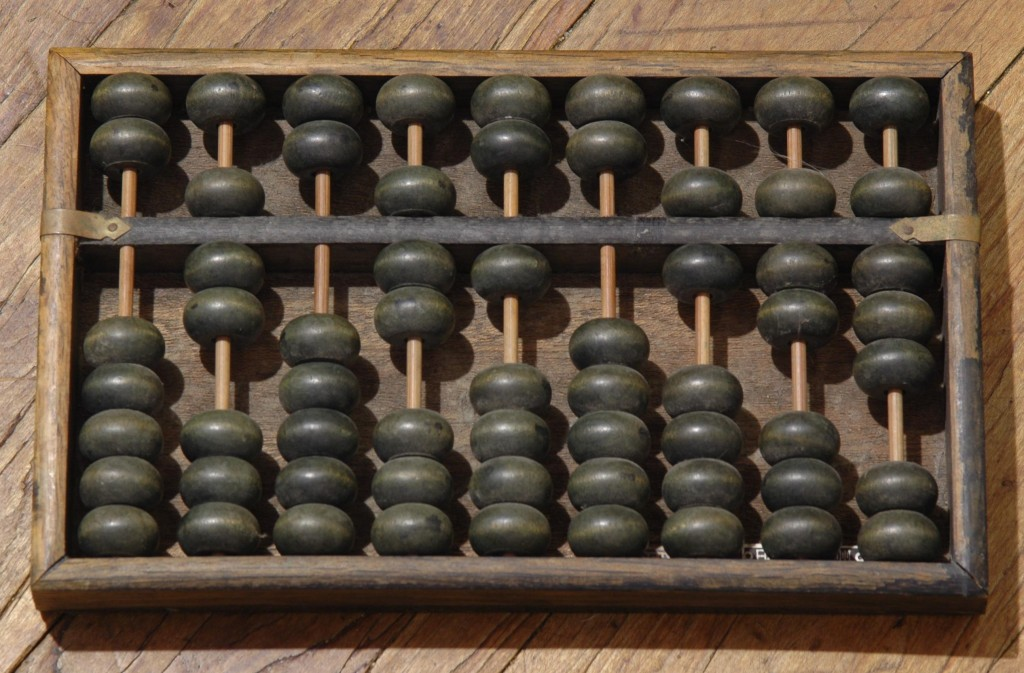
\includegraphics[width=8cm,keepaspectratio=true]{Images/Bouclierimage.jpg}
\hspace{1cm}
\\
\textbf{\caption{Le boulier}}

\end{center}
Le \textbf{boulier} est l’un des premiers outils à calculer, créé en Mésopotamie au \textsc{vii}\textsuperscript{e} siècle avant J.-C. C’est un outil manuel qui permet de faire des calculs élémentaires et qui était composé, à l’époque, d’un contour en bois et d’entassements de cailloux. Le boulier est encore utilisé dans les écoles en Russie et en Chine.


\begin{center}
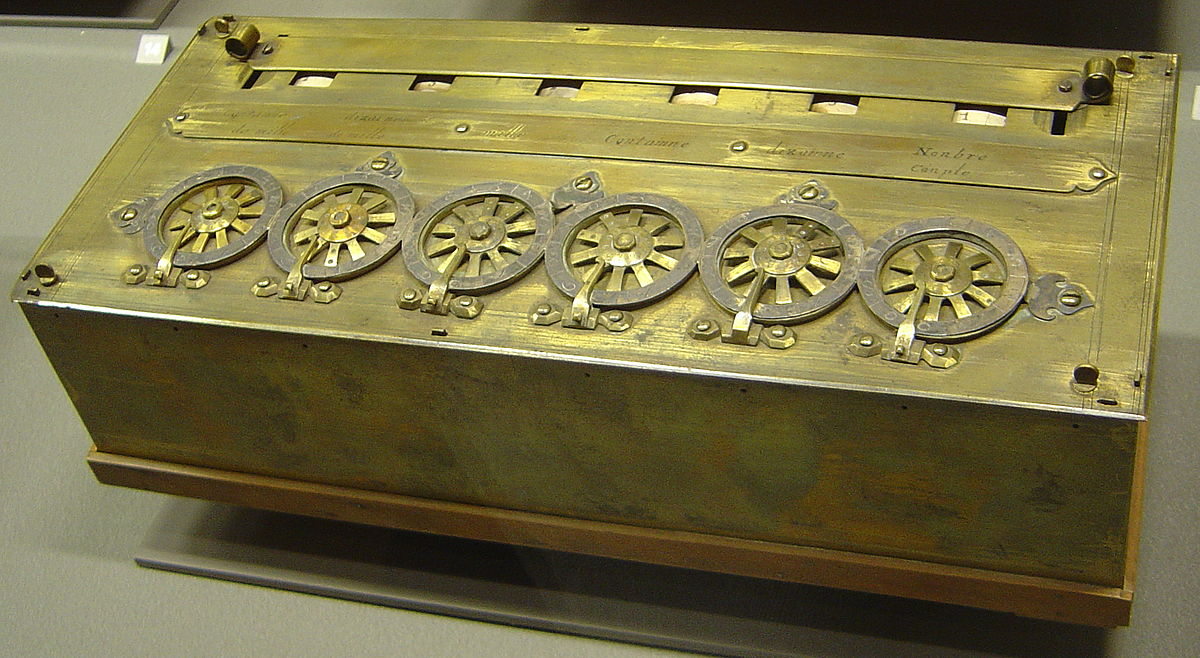
\includegraphics[width=8cm,keepaspectratio=true]{Images/pascaline.jpg}
\hspace{1cm}
\\
\textbf{\caption{La Pascaline}}

\end{center}
La \textbf{Pascaline} est une machine créée par Blaise Pascal en 1642, qui permet d’effectuer des calculs tels que des additions et des soustractions de façon automatique. Elle remplaçait les calculs faits à la main, qui pouvaient être complexes et sujets à erreurs. Blaise Pascal est un mathématicien et philosophe français du \textsc{xvii}\textsuperscript{e} siècle. À cette époque, c’est une invention révolutionnaire qui ouvre la voie aux machines à calculer mécaniques et électroniques. Le principe de la Pascaline est le suivant~: la personne voulant faire une addition ou une soustraction sélectionne les chiffres sur les engrenages, puis la machine effectue le calcul automatiquement. Nous pouvons citer aussi d’autres machines, comme la machine à calculer de Leibniz en 1673, qui s’inspire de la Pascaline. Cette machine permet de multiplier et de diviser, et il existe bien d’autres machines.



\section{Les machines à circuits électriques}

\begin{center}
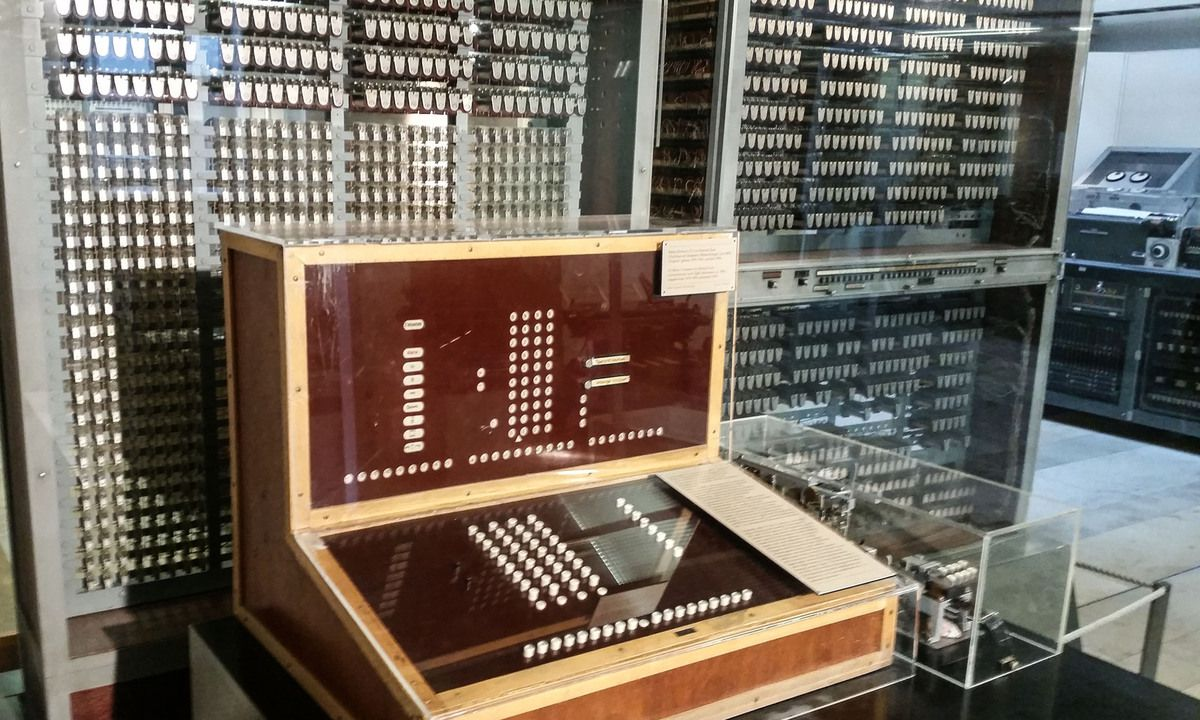
\includegraphics[width=8cm,keepaspectratio=true]{Images/Z3.jpg}
\hspace{1cm}
\\
\textbf{\caption{Z3}}
\end{center}
Pendant la première partie du \textsc{xx}\textsuperscript{e} siècle, l’avancée des mathématiques et de la physique donne un nouveau souffle à la recherche informatique. Celle-ci donna naissance au premier ordinateur programmable, le \textbf{Z3}, créé par l’Allemand Konrad Zuse en 1941, pendant la Seconde Guerre mondiale. C’est le premier ordinateur électromécanique de l’histoire, et il est basé sur des principes logiques. Cet ordinateur réalise une multiplication en 4 secondes en moyenne et il est capable de traiter des nombres à virgule. Cette machine est aussi programmable et était beaucoup utilisée dans le génie civil. Cette invention est l’un des précurseurs des ordinateurs modernes.

\begin{center}
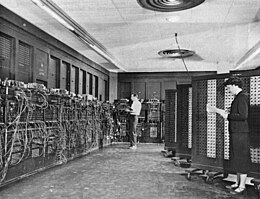
\includegraphics[width=8cm,keepaspectratio=true]{Images/ENIAC.jpg}
\hspace{1cm}
\\
\textbf{\caption{L’ENIAC}}
\end{center}
L’\textbf{ENIAC}, créé en 1944, devient ainsi le premier ordinateur sans aucune pièce mécanique. C’est une très grosse machine qui pesait 30 tonnes, avec 18\,000 tubes à vide~; ces tubes permettaient de le programmer facilement en basculant des interrupteurs. Il est aussi composé de 18\,000 lampes. Lors de l’inauguration de la machine en 1946, par une démonstration, le premier programme est écrit par une femme, ce qui était une première à l’époque. Et l’ENIAC sera utilisé pour fabriquer la première bombe H.



\section{Les premiers ordinateurs personnels}
Cette évolution continue~: la création des transistors, des circuits intégrés et l’apparition de nouveaux langages de programmation réduisent la taille et le coût des ordinateurs. Par exemple, en 1970, les premiers systèmes d’exploitation, dont UNIX, et même la création du premier microprocesseur par Intel facilitent cette évolution.

\begin{center}
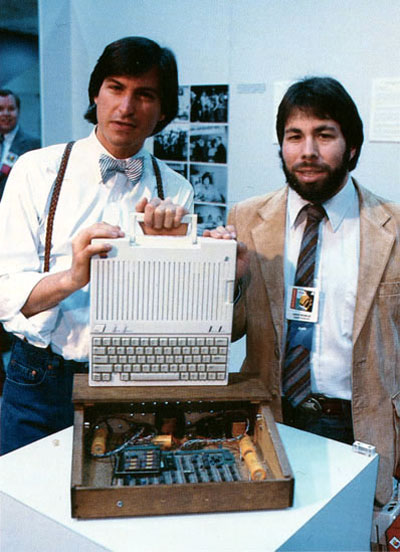
\includegraphics[width=8cm,keepaspectratio=true]{Images/1ordi_apple.jpg}
\hspace{1cm}
\\
\textbf{\caption{Steve Jobs et Steve Wozniak présentent le premier micro-ordinateur d’Apple}}
\end{center}

\begin{center}
    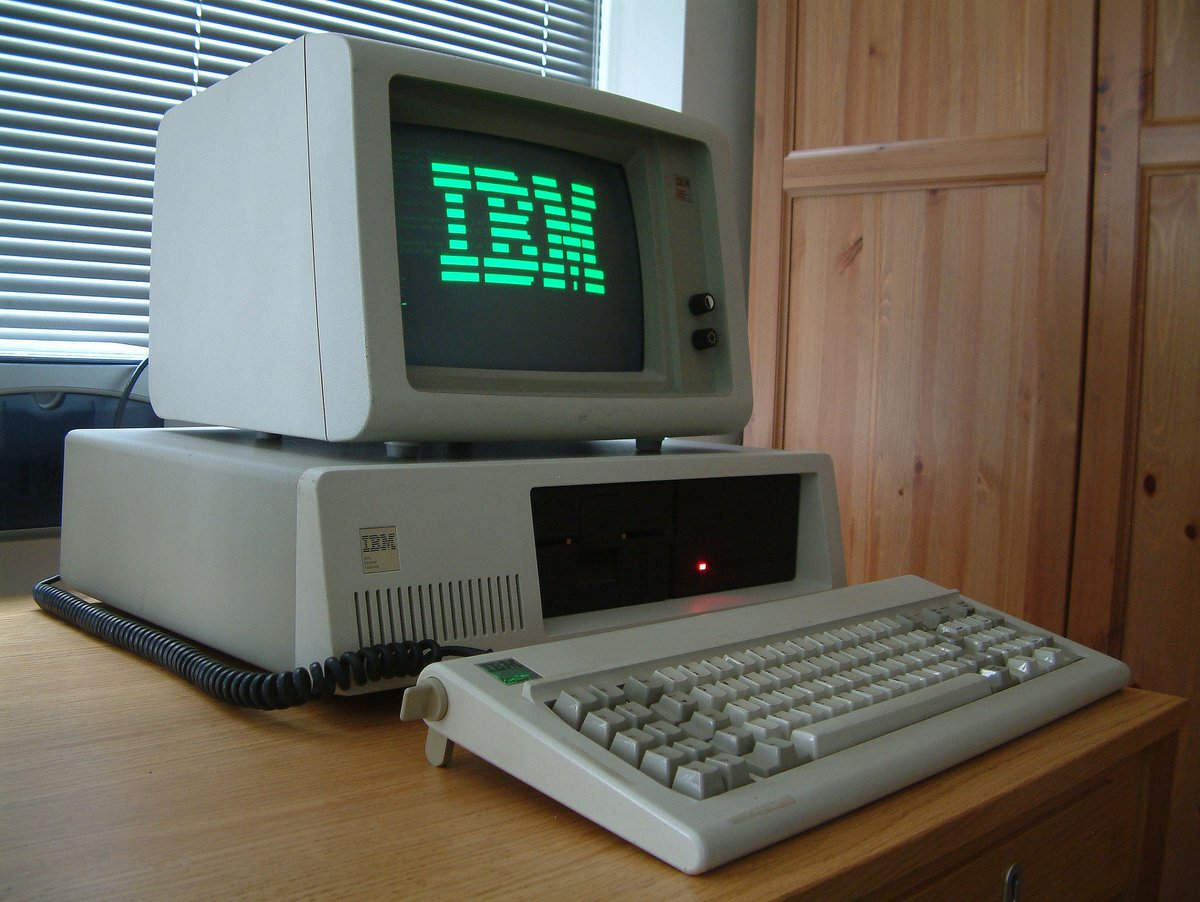
\includegraphics[width=8cm,keepaspectratio=true]{Images/ibm_1pc.jpeg}
    \hspace{1cm}
    \\
    \textbf{\caption{Premier ordinateur personnel d’IBM en 1981}}
\end{center}
Tout cela permet aux foyers d’acheter des ordinateurs personnels familiaux, et la création de jeux sur PC permet une utilisation diverse de l’ordinateur, auparavant privilégié pour des fins professionnelles. Après les années 1990, tout cela s’accélère avec la création de composants informatiques (processeur, carte mère, RAM)~: on parle alors de nanotechnologie.

\begin{center}
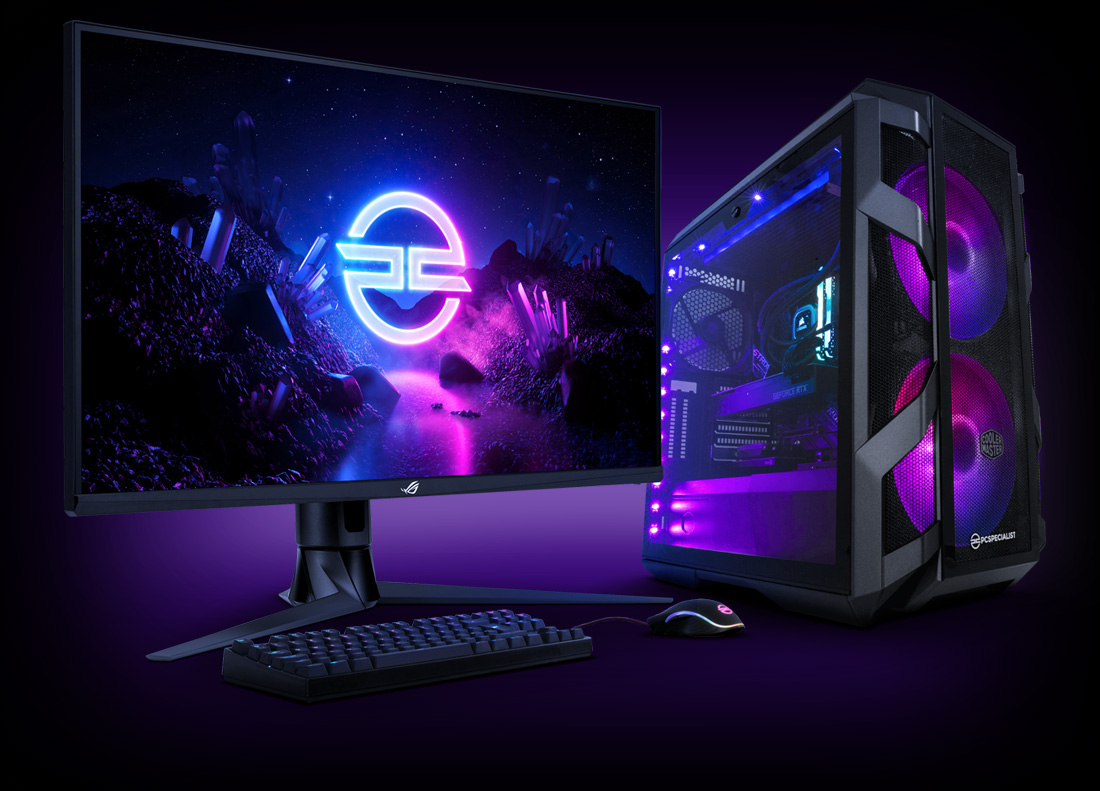
\includegraphics[width=8cm,keepaspectratio=true]{Images/pcgamer.jpg}
\hspace{1cm}
\end{center}



\section{Conclusion}
L’évolution des ordinateurs est une histoire passionnante, marquée par des avancées technologiques extraordinaires, des premiers ordinateurs gigantesques aux ordinateurs personnels. Ils ont radicalement transformé notre façon de travailler, de communiquer, de nous divertir et d’accéder à l’information. À l’avenir, nous pouvons nous attendre à des ordinateurs de plus en plus puissants, qu’il faudra gérer avec précaution. En somme, les ordinateurs continueront d’être des outils indispensables pour stimuler l’innovation et favoriser le progrès humain.


\renewcommand\refname{Références}
\bibliographystyle{plain}
\nocite{1,2,3,4}
\bibliography{rapport}


\end{document}
